% Options for packages loaded elsewhere
\PassOptionsToPackage{unicode}{hyperref}
\PassOptionsToPackage{hyphens}{url}
%
\documentclass[
]{book}
\usepackage{amsmath,amssymb}
\usepackage{lmodern}
\usepackage{iftex}
\ifPDFTeX
  \usepackage[T1]{fontenc}
  \usepackage[utf8]{inputenc}
  \usepackage{textcomp} % provide euro and other symbols
\else % if luatex or xetex
  \usepackage{unicode-math}
  \defaultfontfeatures{Scale=MatchLowercase}
  \defaultfontfeatures[\rmfamily]{Ligatures=TeX,Scale=1}
\fi
% Use upquote if available, for straight quotes in verbatim environments
\IfFileExists{upquote.sty}{\usepackage{upquote}}{}
\IfFileExists{microtype.sty}{% use microtype if available
  \usepackage[]{microtype}
  \UseMicrotypeSet[protrusion]{basicmath} % disable protrusion for tt fonts
}{}
\makeatletter
\@ifundefined{KOMAClassName}{% if non-KOMA class
  \IfFileExists{parskip.sty}{%
    \usepackage{parskip}
  }{% else
    \setlength{\parindent}{0pt}
    \setlength{\parskip}{6pt plus 2pt minus 1pt}}
}{% if KOMA class
  \KOMAoptions{parskip=half}}
\makeatother
\usepackage{xcolor}
\usepackage{longtable,booktabs,array}
\usepackage{calc} % for calculating minipage widths
% Correct order of tables after \paragraph or \subparagraph
\usepackage{etoolbox}
\makeatletter
\patchcmd\longtable{\par}{\if@noskipsec\mbox{}\fi\par}{}{}
\makeatother
% Allow footnotes in longtable head/foot
\IfFileExists{footnotehyper.sty}{\usepackage{footnotehyper}}{\usepackage{footnote}}
\makesavenoteenv{longtable}
\usepackage{graphicx}
\makeatletter
\def\maxwidth{\ifdim\Gin@nat@width>\linewidth\linewidth\else\Gin@nat@width\fi}
\def\maxheight{\ifdim\Gin@nat@height>\textheight\textheight\else\Gin@nat@height\fi}
\makeatother
% Scale images if necessary, so that they will not overflow the page
% margins by default, and it is still possible to overwrite the defaults
% using explicit options in \includegraphics[width, height, ...]{}
\setkeys{Gin}{width=\maxwidth,height=\maxheight,keepaspectratio}
% Set default figure placement to htbp
\makeatletter
\def\fps@figure{htbp}
\makeatother
\setlength{\emergencystretch}{3em} % prevent overfull lines
\providecommand{\tightlist}{%
  \setlength{\itemsep}{0pt}\setlength{\parskip}{0pt}}
\setcounter{secnumdepth}{5}
\ifLuaTeX
\usepackage[bidi=basic]{babel}
\else
\usepackage[bidi=default]{babel}
\fi
\babelprovide[main,import]{brazilian}
% get rid of language-specific shorthands (see #6817):
\let\LanguageShortHands\languageshorthands
\def\languageshorthands#1{}
\usepackage{booktabs}
\usepackage{longtable}
\usepackage{array}
\usepackage{multirow}
\usepackage{wrapfig}
\usepackage{float}
\usepackage{colortbl}
\usepackage{pdflscape}
\usepackage{tabu}
\usepackage{threeparttable}
\usepackage{threeparttablex}
\usepackage[normalem]{ulem}
\usepackage{makecell}
\usepackage{xcolor}
\usepackage{booktabs}
\usepackage{longtable}
\usepackage{array}
\usepackage{multirow}
\usepackage{wrapfig}
\usepackage{float}
\usepackage{colortbl}
\usepackage{pdflscape}
\usepackage{tabu}
\usepackage{threeparttable}
\usepackage{threeparttablex}
\usepackage[normalem]{ulem}
\usepackage{makecell}
\usepackage{xcolor}
\ifLuaTeX
  \usepackage{selnolig}  % disable illegal ligatures
\fi
\usepackage[]{natbib}
\bibliographystyle{plainnat}
\IfFileExists{bookmark.sty}{\usepackage{bookmark}}{\usepackage{hyperref}}
\IfFileExists{xurl.sty}{\usepackage{xurl}}{} % add URL line breaks if available
\urlstyle{same} % disable monospaced font for URLs
\hypersetup{
  pdftitle={Bookdown Resumos de Matemática 2},
  pdfauthor={Daniel Claudino},
  pdflang={pt-BR},
  hidelinks,
  pdfcreator={LaTeX via pandoc}}

\title{Bookdown Resumos de Matemática 2}
\author{Daniel Claudino}
\date{2022-12-11}

\begin{document}
\maketitle

{
\setcounter{tocdepth}{1}
\tableofcontents
}
\hypertarget{apresentauxe7uxe3o}{%
\chapter{Apresentação}\label{apresentauxe7uxe3o}}

Bookdown Resumos de Matemática 2

\begin{figure}

{\centering 
\includegraphics[width=0.5\linewidth]{imagens/FOTO-PERFIL-DANIEL-CLAUDINO-2020} 

}

\caption{Autor}\label{fig:unnamed-chunk-1}
\end{figure}

\begin{itemize}
\tightlist
\item
  Neste material, estão contidos resumos de matemática 2.
\end{itemize}

\hypertarget{controle-de-versuxe3o}{%
\section{Controle de Versão}\label{controle-de-versuxe3o}}

\begin{longtable}[]{@{}
  >{\raggedright\arraybackslash}p{(\columnwidth - 6\tabcolsep) * \real{0.2500}}
  >{\raggedright\arraybackslash}p{(\columnwidth - 6\tabcolsep) * \real{0.2500}}
  >{\raggedright\arraybackslash}p{(\columnwidth - 6\tabcolsep) * \real{0.2500}}
  >{\raggedright\arraybackslash}p{(\columnwidth - 6\tabcolsep) * \real{0.2500}}@{}}
\toprule()
\begin{minipage}[b]{\linewidth}\raggedright
Versão
\end{minipage} & \begin{minipage}[b]{\linewidth}\raggedright
Data / Hora
\end{minipage} & \begin{minipage}[b]{\linewidth}\raggedright
Colaborador
\end{minipage} & \begin{minipage}[b]{\linewidth}\raggedright
Descrição da Contribuição
\end{minipage} \\
\midrule()
\endhead
0.1 & dd/mm/aaaa xxh00 & \href{https://wa.me/5583988853815}{Daniel Claudino} & Versão inicial do documento \\
\bottomrule()
\end{longtable}

\hypertarget{anuxe1lise-combinatuxf3ria-manoel-paiva-vol-2-2004}{%
\chapter{Análise Combinatória (Manoel Paiva, Vol 2, 2004)}\label{anuxe1lise-combinatuxf3ria-manoel-paiva-vol-2-2004}}

Neste capítulo estarão contidos os resumos de \textbf{Análise Combinatória} de do livro de Matemática - Volume 2, do autor Manoel Paiva, 1º edição, 2004, da editora Moderna.

\begin{figure}

{\centering 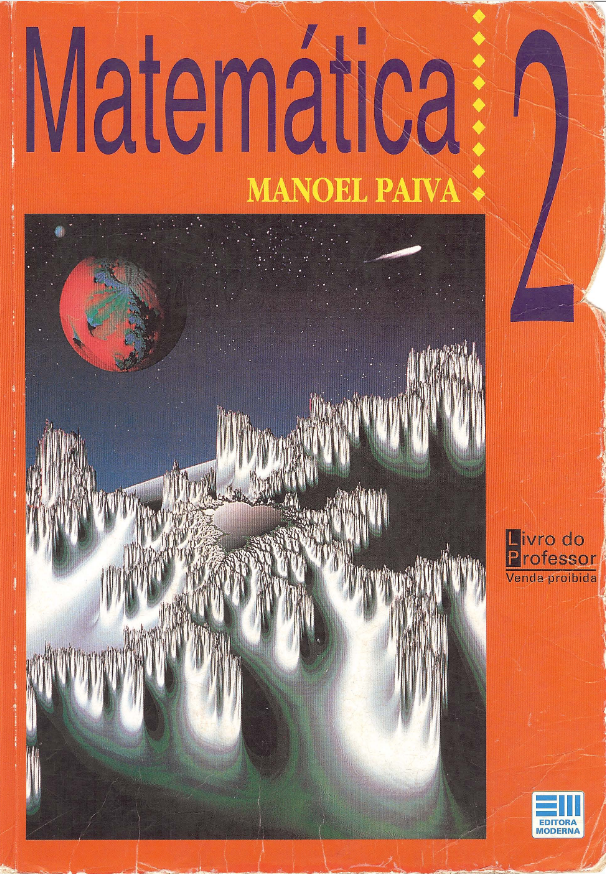
\includegraphics[width=0.5\linewidth]{imagens/Capa-Livro-Matematica-Volume-2-Manoel-Paiva-2004} 

}

\caption{Livro - Matemática Vol 3 - Manoel Paiva, 2004 (Ed. Moderna, 1.ed.)}\label{fig:carregaImagemCapaLivro}
\end{figure}

\begin{longtable}[]{@{}cc@{}}
\toprule()
Capítulo & Descrição \\
\midrule()
\endhead
21 & Análise combinatória - métodos de contagem \\
22 & Princípio aditivo da contagem \\
23 & Arranjo simples \\
24 & Fatorial \\
25 & Permutação simples \\
26 & Permutação com elementos repetidos \\
27 & Combinação simples \\
27-X & Combinação com elementos Repetidos \\
28 & Permutação circular \\
\bottomrule()
\end{longtable}

\hypertarget{capuxedtulo-21---anuxe1lise-combinatuxf3ria-muxe9todos-de-contagem}{%
\section{Capítulo 21 - Análise combinatória (Métodos de contagem)}\label{capuxedtulo-21---anuxe1lise-combinatuxf3ria-muxe9todos-de-contagem}}

\hypertarget{introduuxe7uxe3o}{%
\subsection{Introdução}\label{introduuxe7uxe3o}}

Contar é uma necessidade cotidiana. Contamos a quantidade de frutas em um cesto, a quantidade de livros em uma estante, a quantidade de habitantes em uma cidade, etc.

Existem quantidades que não são tão fáceis de contar tais como quantos números de telefones que podemos obter com 8 dígitos, a quantidade de placas de automóveis que podemos obter com 3 letras seguidas de 4 algarismos.

A análise combinatória é a parte da matemática que estabelece métodos para contar nesses casos mais difíceis (\textbf{métodos de contagem}).

\hypertarget{princuxedpio-fundamental-da-contagem}{%
\subsection{Princípio Fundamental da Contagem}\label{princuxedpio-fundamental-da-contagem}}

SE um experimento \textbf{A} apresenta \textbf{n} resultados distintos e um experimento \textbf{B} apresenta \textbf{k} resultados distintos, ENTÃO o experimento composto \textbf{A e B}, nessa ordem, apresenta \(n \times k\) resultados distintos.

\hypertarget{exemplos-de-experimentos}{%
\subsubsection*{Exemplos de Experimentos}\label{exemplos-de-experimentos}}
\addcontentsline{toc}{subsubsection}{Exemplos de Experimentos}

\begin{enumerate}
\def\labelenumi{\arabic{enumi}.}
\tightlist
\item
  Jogar um dado de 6 lados (Experimento simples: 1 experimento);
\item
  Jogar uma moeda (Experimento simples: 1 experimento);
\item
  Jogar um dado de 6 lados e em seguinda jogar uma moeda, nessa ordem (Experimento composto: 2 experimentos);
\item
  Jogar um dado de 6 lados, uma moeda e em seguida retirar uma bola de uma urna com 4 bolas das cores vermelho, preto, azul e amarela (Experimento composto: 3 experimentos);
\end{enumerate}

\hypertarget{formas-de-demonstrar-experimentos}{%
\subsubsection*{Formas de Demonstrar Experimentos}\label{formas-de-demonstrar-experimentos}}
\addcontentsline{toc}{subsubsection}{Formas de Demonstrar Experimentos}

\hypertarget{matruxedz-de-possibilidades}{%
\paragraph{Matríz de Possibilidades}\label{matruxedz-de-possibilidades}}

Podemos demonstrar todos os resultados possíveis de um experimento simples ou composto construindo uma uma matriz de possibilidades.

\hypertarget{experimento-simples}{%
\subparagraph{Experimento Simples}\label{experimento-simples}}

Para um \textbf{experimento simples} de jogar um dado de 6 faces:

\begin{table}

\caption{\label{tab:tabela3}Exemplo - Resultados possíveis do Experimento - Jogar um dado de 6 faces}
\centering
\begin{tabular}[t]{l}
\toprule
Jogada\\
\midrule
\cellcolor{gray!6}{Face 1}\\
Face 2\\
\cellcolor{gray!6}{Face 3}\\
Face 4\\
\cellcolor{gray!6}{Face 5}\\
\addlinespace
Face 6\\
\bottomrule
\multicolumn{1}{l}{\rule{0pt}{1em}\textit{Fonte: } Paiva (2004, pág. 154)}\\
\end{tabular}
\end{table}

\hypertarget{experimento-composto-dois-experimentos}{%
\subparagraph{Experimento Composto ( dois experimentos )}\label{experimento-composto-dois-experimentos}}

Para um \textbf{experimento composto}, contendo dois experimentos: (A) Jogar um dado de 6 faces e (B) jogar uma moeda.

\begin{enumerate}
\def\labelenumi{\arabic{enumi}.}
\tightlist
\item
  Construímos uma matriz com as \textbf{n} linhas contendo os elementos do experimento \textbf{A};
\item
  Adicionamos \textbf{k} colunas contendo os elementos do experimento \textbf{B}.
\end{enumerate}

\begin{table}

\caption{\label{tab:tabela1}Exemplo - Resultado do Experimento - Jogar um dado de 6 faces e jogar uma moeda}
\centering
\begin{tabular}[t]{lll}
\toprule
ExperimentoA & ExperimentoB.C. & ExperimentoB.K.\\
\midrule
\cellcolor{gray!6}{Face 1} & \cellcolor{gray!6}{( 1 , C )} & \cellcolor{gray!6}{( 1 , K )}\\
Face 2 & ( 2 , C ) & ( 2 , K )\\
\cellcolor{gray!6}{Face 3} & \cellcolor{gray!6}{( 3 , C )} & \cellcolor{gray!6}{( 3 , K )}\\
Face 4 & ( 4 , C ) & ( 4 , K )\\
\cellcolor{gray!6}{Face 5} & \cellcolor{gray!6}{( 5 , C )} & \cellcolor{gray!6}{( 5 , K )}\\
\addlinespace
Face 6 & ( 6 , C ) & ( 6 , K )\\
\bottomrule
\multicolumn{3}{l}{\rule{0pt}{1em}\textit{Fonte: } Paiva (2004, pág. 154)}\\
\end{tabular}
\end{table}

Logo, os resultados possíveis são:

\begin{table}

\caption{\label{tab:unnamed-chunk-2}Exemplo - Lista de Resultados do Experimento - Jogar um dado de 6 faces e jogar uma moeda}
\centering
\begin{tabular}[t]{l}
\toprule
Resultados\\
\midrule
\cellcolor{gray!6}{( 1 , C )}\\
( 2 , C )\\
\cellcolor{gray!6}{( 3 , C )}\\
( 4 , C )\\
\cellcolor{gray!6}{( 5 , C )}\\
\addlinespace
( 6 , C )\\
\cellcolor{gray!6}{( 1 , K )}\\
( 2 , K )\\
\cellcolor{gray!6}{( 3 , K )}\\
( 4 , K )\\
\addlinespace
\cellcolor{gray!6}{( 5 , K )}\\
( 6 , K )\\
\bottomrule
\multicolumn{1}{l}{\rule{0pt}{1em}\textit{Fonte: } Paiva (2004, pág. 154)}\\
\end{tabular}
\end{table}

\hypertarget{experimento-composto-truxeas-experimentos}{%
\subparagraph{Experimento Composto ( três experimentos )}\label{experimento-composto-truxeas-experimentos}}

Vamos supor que o experimento seja composto de \textbf{três experimentos}, qual sejam (A) jogar um dado de 6 faces, (B) jogar uma moeda e (C) retirar uma bola de uma urna contendo quatro bolas (preto, azul, verde, vermelha).

\begin{enumerate}
\def\labelenumi{\arabic{enumi}.}
\tightlist
\item
  Construímos a matriz de possibilidades entre o 1º e 2º experimentos:
\end{enumerate}

\begin{table}

\caption{\label{tab:unnamed-chunk-3}Matriz de possibilidades com os resultados possíveis entre o 1º e 2º experimentos}
\centering
\begin{tabular}[t]{lll}
\toprule
JogarDado & ExperimentoB.C. & ExperimentoB.K.\\
\midrule
\cellcolor{gray!6}{Face 1} & \cellcolor{gray!6}{( 1 , C )} & \cellcolor{gray!6}{( 1 , K )}\\
Face 2 & ( 2 , C ) & ( 2 , K )\\
\cellcolor{gray!6}{Face 3} & \cellcolor{gray!6}{( 3 , C )} & \cellcolor{gray!6}{( 3 , K )}\\
Face 4 & ( 4 , C ) & ( 4 , K )\\
\cellcolor{gray!6}{Face 5} & \cellcolor{gray!6}{( 5 , C )} & \cellcolor{gray!6}{( 5 , K )}\\
\addlinespace
Face 6 & ( 6 , C ) & ( 6 , K )\\
\bottomrule
\multicolumn{3}{l}{\rule{0pt}{1em}\textit{Fonte: } Paiva (2004, pág. 155)}\\
\end{tabular}
\end{table}

\begin{enumerate}
\def\labelenumi{\arabic{enumi}.}
\setcounter{enumi}{1}
\tightlist
\item
  Listar os resultados possíveis da matriz de possibilidades:
\end{enumerate}

\begin{table}

\caption{\label{tab:unnamed-chunk-4}Lista de Resultados do Experimento - Jogar um dado de 6 faces e jogar uma moeda}
\centering
\begin{tabular}[t]{l}
\toprule
Resultados\\
\midrule
\cellcolor{gray!6}{( 1 , C )}\\
( 2 , C )\\
\cellcolor{gray!6}{( 3 , C )}\\
( 4 , C )\\
\cellcolor{gray!6}{( 5 , C )}\\
\addlinespace
( 6 , C )\\
\cellcolor{gray!6}{( 1 , K )}\\
( 2 , K )\\
\cellcolor{gray!6}{( 3 , K )}\\
( 4 , K )\\
\addlinespace
\cellcolor{gray!6}{( 5 , K )}\\
( 6 , K )\\
\bottomrule
\multicolumn{1}{l}{\rule{0pt}{1em}\textit{Fonte: } Paiva (2004, pág. 154)}\\
\end{tabular}
\end{table}

\begin{enumerate}
\def\labelenumi{\arabic{enumi}.}
\setcounter{enumi}{2}
\tightlist
\item
  Listar os resultados possíves do 3º subexperimento (Retirar bola de urna)
\end{enumerate}

\begin{table}

\caption{\label{tab:unnamed-chunk-5}Lista de Resultados do Experimento - Retirar uma bola de uma urna contendo quatro bolas (preto, azul, amarela, vermelha).}
\centering
\begin{tabular}[t]{l}
\toprule
RetirarBolaDeUrna\\
\midrule
\cellcolor{gray!6}{Bola preta}\\
Bola azul\\
\cellcolor{gray!6}{Bola amarela}\\
Bola vermelha\\
\bottomrule
\multicolumn{1}{l}{\rule{0pt}{1em}\textit{Fonte: } Paiva (2004, pág. 154)}\\
\end{tabular}
\end{table}

\begin{enumerate}
\def\labelenumi{\arabic{enumi}.}
\setcounter{enumi}{3}
\tightlist
\item
  Construir uma matriz com \textbf{n} linhas da lista do item 2 por \textbf{k} colunas da lista do item 3
\end{enumerate}

\begin{table}

\caption{\label{tab:unnamed-chunk-6}Lista de Resultados do Experimento - Jogar um dado de 6 faces e jogar uma moeda}
\centering
\begin{tabular}[t]{lllll}
\toprule
ResultadosExperimentos1E2 & BolaAmarela & BolaVerde & BolaPreta & BolaBranca\\
\midrule
\cellcolor{gray!6}{(1, C)} & \cellcolor{gray!6}{(1, C, A)} & \cellcolor{gray!6}{(1, C, V)} & \cellcolor{gray!6}{(1, C, P)} & \cellcolor{gray!6}{(1, C, B)}\\
(1, K) & (1, K, A) & (1, K, V) & (1, K, P) & (1, K, B)\\
\cellcolor{gray!6}{(2, C)} & \cellcolor{gray!6}{(2, C, A)} & \cellcolor{gray!6}{(2, C, V)} & \cellcolor{gray!6}{(2, C, P)} & \cellcolor{gray!6}{(2, C, B)}\\
(2, K) & (2, K, A) & (2, K, V) & (2, K, P) & (2, K, B)\\
\cellcolor{gray!6}{(3, C)} & \cellcolor{gray!6}{(3, C, A)} & \cellcolor{gray!6}{(3, C, V)} & \cellcolor{gray!6}{(3, C, P)} & \cellcolor{gray!6}{(3, C, B)}\\
\addlinespace
(3, K) & (3, K, A) & (3, K, V) & (3, K, P) & (3, K, B)\\
\cellcolor{gray!6}{(4, C)} & \cellcolor{gray!6}{(4, C, A)} & \cellcolor{gray!6}{(4, C, V)} & \cellcolor{gray!6}{(4, C, P)} & \cellcolor{gray!6}{(4, C, B)}\\
(4, K) & (4, K, A) & (4, K, V) & (4, K, P) & (4, K, B)\\
\cellcolor{gray!6}{(5, C)} & \cellcolor{gray!6}{(5, C, A)} & \cellcolor{gray!6}{(5, C, V)} & \cellcolor{gray!6}{(5, C, P)} & \cellcolor{gray!6}{(5, C, B)}\\
(5, K) & (5, K, A) & (5, K, V) & (5, K, P) & (5, K, B)\\
\addlinespace
\cellcolor{gray!6}{(6, C)} & \cellcolor{gray!6}{(6, C, A)} & \cellcolor{gray!6}{(6, C, V)} & \cellcolor{gray!6}{(6, C, P)} & \cellcolor{gray!6}{(6, C, B)}\\
(6, K) & (6, K, A) & (6, K, V) & (6, K, P) & (6, K, B)\\
\bottomrule
\multicolumn{5}{l}{\rule{0pt}{1em}\textit{Fonte: } Paiva (2004, pág. 154)}\\
\end{tabular}
\end{table}

\begin{enumerate}
\def\labelenumi{\arabic{enumi}.}
\setcounter{enumi}{4}
\tightlist
\item
  Repetir os procedimentos de 1 a 4, caso hajam mais experimentos (4º, 5º, 6º, etc.)
\end{enumerate}

\hypertarget{uxe1rvore-de-possibilidades}{%
\paragraph{Árvore de Possibilidades}\label{uxe1rvore-de-possibilidades}}

Podemos demonstrar todos os resultados possíveis de um experimento através de uma árvore de possibilidades.

\begin{verbatim}
## PhantomJS not found. You can install it with webshot::install_phantomjs(). If it is installed, please make sure the phantomjs executable can be found via the PATH variable.
\end{verbatim}

\hypertarget{generalizauxe7uxe3o-do-princuxedpio-fundamental-da-contagem}{%
\subsection{Generalização do Princípio Fundamental da Contagem}\label{generalizauxe7uxe3o-do-princuxedpio-fundamental-da-contagem}}

Se os experimentos \(A_{1}, A_{2}, A_{3}, ..., A_{k}\) apresentam como número de resultados possíveis, respectivamente, \(n_{1}, n_{2}, n_{3}, ..., n_{k}\), então o \textbf{experimento composto} \(A_{1}, A_{2}, A_{3}, ..., A_{k}\), nessa ordem, apresenta \(n_{1} \times n_{2} \times n_{3} \times ... \times n_{k}\) resultados possíveis.

\hypertarget{exercuxedcios}{%
\subsection*{Exercícios}\label{exercuxedcios}}
\addcontentsline{toc}{subsection}{Exercícios}

\hypertarget{capuxedtulo-22---princuxedpio-aditivo-da-contagem}{%
\section{Capítulo 22 - Princípio aditivo da contagem}\label{capuxedtulo-22---princuxedpio-aditivo-da-contagem}}

\hypertarget{subseuxe7uxe3o-numerada-1}{%
\subsection{Subseção Numerada 1}\label{subseuxe7uxe3o-numerada-1}}

Lorem ipsum. Lorem ipsum. Lorem ipsum. Lorem ipsum. Lorem ipsum. Lorem ipsum. Lorem ipsum. Lorem ipsum. Lorem ipsum. Lorem ipsum. Lorem ipsum. Lorem ipsum. Lorem ipsum. Lorem ipsum. Lorem ipsum. Lorem ipsum. Lorem ipsum. Lorem ipsum. Lorem ipsum.

\hypertarget{exercuxedcios-do-capuxedtulo-22}{%
\subsection{Exercícios do Capítulo 22}\label{exercuxedcios-do-capuxedtulo-22}}

Lorem ipsum. Lorem ipsum. Lorem ipsum. Lorem ipsum. Lorem ipsum. Lorem ipsum. Lorem ipsum. Lorem ipsum. Lorem ipsum. Lorem ipsum. Lorem ipsum. Lorem ipsum. Lorem ipsum. Lorem ipsum. Lorem ipsum. Lorem ipsum. Lorem ipsum. Lorem ipsum. Lorem ipsum.

\hypertarget{seuxe7uxe3o-nuxe3o-numerada-3}{%
\subsection*{Seção não Numerada 3}\label{seuxe7uxe3o-nuxe3o-numerada-3}}
\addcontentsline{toc}{subsection}{Seção não Numerada 3}

Lorem ipsum. Lorem ipsum. Lorem ipsum. Lorem ipsum. Lorem ipsum. Lorem ipsum. Lorem ipsum. Lorem ipsum. Lorem ipsum. Lorem ipsum. Lorem ipsum. Lorem ipsum. Lorem ipsum. Lorem ipsum. Lorem ipsum. Lorem ipsum. Lorem ipsum. Lorem ipsum. Lorem ipsum.

\hypertarget{capuxedtulo-23---arranjo-simples}{%
\section{Capítulo 23 - Arranjo simples}\label{capuxedtulo-23---arranjo-simples}}

\hypertarget{subseuxe7uxe3o-numerada-1-1}{%
\subsection{Subseção Numerada 1}\label{subseuxe7uxe3o-numerada-1-1}}

Lorem ipsum. Lorem ipsum. Lorem ipsum. Lorem ipsum. Lorem ipsum. Lorem ipsum. Lorem ipsum. Lorem ipsum. Lorem ipsum. Lorem ipsum. Lorem ipsum. Lorem ipsum. Lorem ipsum. Lorem ipsum. Lorem ipsum. Lorem ipsum. Lorem ipsum. Lorem ipsum. Lorem ipsum.

\hypertarget{exercuxedcios-do-capuxedtulo-23}{%
\subsection{Exercícios do Capítulo 23}\label{exercuxedcios-do-capuxedtulo-23}}

Lorem ipsum. Lorem ipsum. Lorem ipsum. Lorem ipsum. Lorem ipsum. Lorem ipsum. Lorem ipsum. Lorem ipsum. Lorem ipsum. Lorem ipsum. Lorem ipsum. Lorem ipsum. Lorem ipsum. Lorem ipsum. Lorem ipsum. Lorem ipsum. Lorem ipsum. Lorem ipsum. Lorem ipsum.

\hypertarget{seuxe7uxe3o-nuxe3o-numerada-3-1}{%
\subsection*{Seção não Numerada 3}\label{seuxe7uxe3o-nuxe3o-numerada-3-1}}
\addcontentsline{toc}{subsection}{Seção não Numerada 3}

Lorem ipsum. Lorem ipsum. Lorem ipsum. Lorem ipsum. Lorem ipsum. Lorem ipsum. Lorem ipsum. Lorem ipsum. Lorem ipsum. Lorem ipsum. Lorem ipsum. Lorem ipsum. Lorem ipsum. Lorem ipsum. Lorem ipsum. Lorem ipsum. Lorem ipsum. Lorem ipsum. Lorem ipsum.

\hypertarget{binuxf4mio-de-newton-manoel-paiva-vol-2-2004}{%
\chapter{Binômio de Newton (Manoel Paiva, Vol 2, 2004)}\label{binuxf4mio-de-newton-manoel-paiva-vol-2-2004}}

Neste capítulo estarão contidos os resumos de \textbf{Binômio de Newton} de do livro de Matemática - Volume 2, do autor Manoel Paiva, 1º edição, 2004, da editora Moderna.

\begin{figure}

{\centering 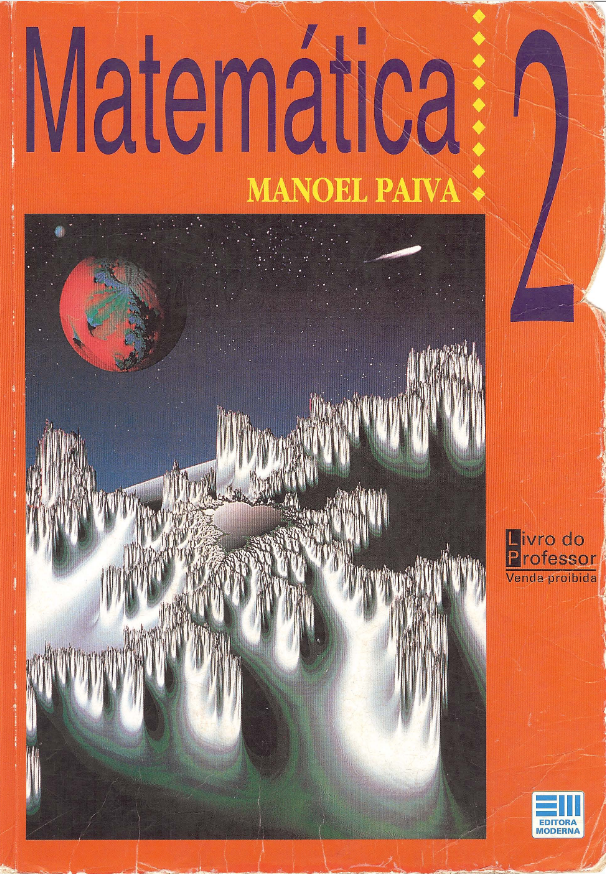
\includegraphics[width=0.5\linewidth]{imagens/Capa-Livro-Matematica-Volume-2-Manoel-Paiva-2004} 

}

\caption{Livro - Matemática Vol 3 - Manoel Paiva, 2004 (Ed. Moderna, 1.ed.)}\label{fig:unnamed-chunk-8}
\end{figure}

\begin{longtable}[]{@{}ll@{}}
\toprule()
Capítulo & Descrição \\
\midrule()
\endhead
29 & Numero binominal \\
30 & Binômio de Newton \\
31 & Termo Geral do Binômio de Newton \\
\bottomrule()
\end{longtable}

\hypertarget{capuxedtulo-21---anuxe1lise-combinatuxf3ria-muxe9todos-de-contagem-1}{%
\section{Capítulo 21 - Análise combinatória (Métodos de contagem)}\label{capuxedtulo-21---anuxe1lise-combinatuxf3ria-muxe9todos-de-contagem-1}}

\hypertarget{subseuxe7uxe3o-numerada-1-2}{%
\subsection{Subseção Numerada 1}\label{subseuxe7uxe3o-numerada-1-2}}

Lorem ipsum. Lorem ipsum. Lorem ipsum. Lorem ipsum. Lorem ipsum. Lorem ipsum. Lorem ipsum. Lorem ipsum. Lorem ipsum. Lorem ipsum. Lorem ipsum. Lorem ipsum. Lorem ipsum. Lorem ipsum. Lorem ipsum. Lorem ipsum. Lorem ipsum. Lorem ipsum. Lorem ipsum.

\hypertarget{exercuxedcios-do-capuxedtulo-21}{%
\subsection{Exercícios do Capítulo 21}\label{exercuxedcios-do-capuxedtulo-21}}

Lorem ipsum. Lorem ipsum. Lorem ipsum. Lorem ipsum. Lorem ipsum. Lorem ipsum. Lorem ipsum. Lorem ipsum. Lorem ipsum. Lorem ipsum. Lorem ipsum. Lorem ipsum. Lorem ipsum. Lorem ipsum. Lorem ipsum. Lorem ipsum. Lorem ipsum. Lorem ipsum. Lorem ipsum.

\hypertarget{seuxe7uxe3o-nuxe3o-numerada-3-2}{%
\subsection*{Seção não Numerada 3}\label{seuxe7uxe3o-nuxe3o-numerada-3-2}}
\addcontentsline{toc}{subsection}{Seção não Numerada 3}

Lorem ipsum. Lorem ipsum. Lorem ipsum. Lorem ipsum. Lorem ipsum. Lorem ipsum. Lorem ipsum. Lorem ipsum. Lorem ipsum. Lorem ipsum. Lorem ipsum. Lorem ipsum. Lorem ipsum. Lorem ipsum. Lorem ipsum. Lorem ipsum. Lorem ipsum. Lorem ipsum. Lorem ipsum.
eção 02

\hypertarget{capuxedtulo-22---princuxedpio-aditivo-da-contagem-1}{%
\section{Capítulo 22 - Princípio aditivo da contagem}\label{capuxedtulo-22---princuxedpio-aditivo-da-contagem-1}}

\hypertarget{subseuxe7uxe3o-numerada-1-3}{%
\subsection{Subseção Numerada 1}\label{subseuxe7uxe3o-numerada-1-3}}

Lorem ipsum. Lorem ipsum. Lorem ipsum. Lorem ipsum. Lorem ipsum. Lorem ipsum. Lorem ipsum. Lorem ipsum. Lorem ipsum. Lorem ipsum. Lorem ipsum. Lorem ipsum. Lorem ipsum. Lorem ipsum. Lorem ipsum. Lorem ipsum. Lorem ipsum. Lorem ipsum. Lorem ipsum.

\hypertarget{exercuxedcios-do-capuxedtulo-22-1}{%
\subsection{Exercícios do Capítulo 22}\label{exercuxedcios-do-capuxedtulo-22-1}}

Lorem ipsum. Lorem ipsum. Lorem ipsum. Lorem ipsum. Lorem ipsum. Lorem ipsum. Lorem ipsum. Lorem ipsum. Lorem ipsum. Lorem ipsum. Lorem ipsum. Lorem ipsum. Lorem ipsum. Lorem ipsum. Lorem ipsum. Lorem ipsum. Lorem ipsum. Lorem ipsum. Lorem ipsum.

\hypertarget{seuxe7uxe3o-nuxe3o-numerada-3-3}{%
\subsection*{Seção não Numerada 3}\label{seuxe7uxe3o-nuxe3o-numerada-3-3}}
\addcontentsline{toc}{subsection}{Seção não Numerada 3}

Lorem ipsum. Lorem ipsum. Lorem ipsum. Lorem ipsum. Lorem ipsum. Lorem ipsum. Lorem ipsum. Lorem ipsum. Lorem ipsum. Lorem ipsum. Lorem ipsum. Lorem ipsum. Lorem ipsum. Lorem ipsum. Lorem ipsum. Lorem ipsum. Lorem ipsum. Lorem ipsum. Lorem ipsum.

\hypertarget{capuxedtulo-23---arranjo-simples-1}{%
\section{Capítulo 23 - Arranjo simples}\label{capuxedtulo-23---arranjo-simples-1}}

\hypertarget{subseuxe7uxe3o-numerada-1-4}{%
\subsection{Subseção Numerada 1}\label{subseuxe7uxe3o-numerada-1-4}}

Lorem ipsum. Lorem ipsum. Lorem ipsum. Lorem ipsum. Lorem ipsum. Lorem ipsum. Lorem ipsum. Lorem ipsum. Lorem ipsum. Lorem ipsum. Lorem ipsum. Lorem ipsum. Lorem ipsum. Lorem ipsum. Lorem ipsum. Lorem ipsum. Lorem ipsum. Lorem ipsum. Lorem ipsum.

\hypertarget{exercuxedcios-do-capuxedtulo-23-1}{%
\subsection{Exercícios do Capítulo 23}\label{exercuxedcios-do-capuxedtulo-23-1}}

Lorem ipsum. Lorem ipsum. Lorem ipsum. Lorem ipsum. Lorem ipsum. Lorem ipsum. Lorem ipsum. Lorem ipsum. Lorem ipsum. Lorem ipsum. Lorem ipsum. Lorem ipsum. Lorem ipsum. Lorem ipsum. Lorem ipsum. Lorem ipsum. Lorem ipsum. Lorem ipsum. Lorem ipsum.

\hypertarget{seuxe7uxe3o-nuxe3o-numerada-3-4}{%
\subsection*{Seção não Numerada 3}\label{seuxe7uxe3o-nuxe3o-numerada-3-4}}
\addcontentsline{toc}{subsection}{Seção não Numerada 3}

Lorem ipsum. Lorem ipsum. Lorem ipsum. Lorem ipsum. Lorem ipsum. Lorem ipsum. Lorem ipsum. Lorem ipsum. Lorem ipsum. Lorem ipsum. Lorem ipsum. Lorem ipsum. Lorem ipsum. Lorem ipsum. Lorem ipsum. Lorem ipsum. Lorem ipsum. Lorem ipsum. Lorem ipsum.

\hypertarget{probabilidade-manoel-paiva-vol-2-2004}{%
\chapter{Probabilidade (Manoel Paiva, Vol 2, 2004)}\label{probabilidade-manoel-paiva-vol-2-2004}}

Neste capítulo estarão contidos os resumos de \textbf{Probabilidade} de do livro de Matemática - Volume 2, do autor Manoel Paiva, 1º edição, 2004, da editora Moderna.

\begin{figure}

{\centering 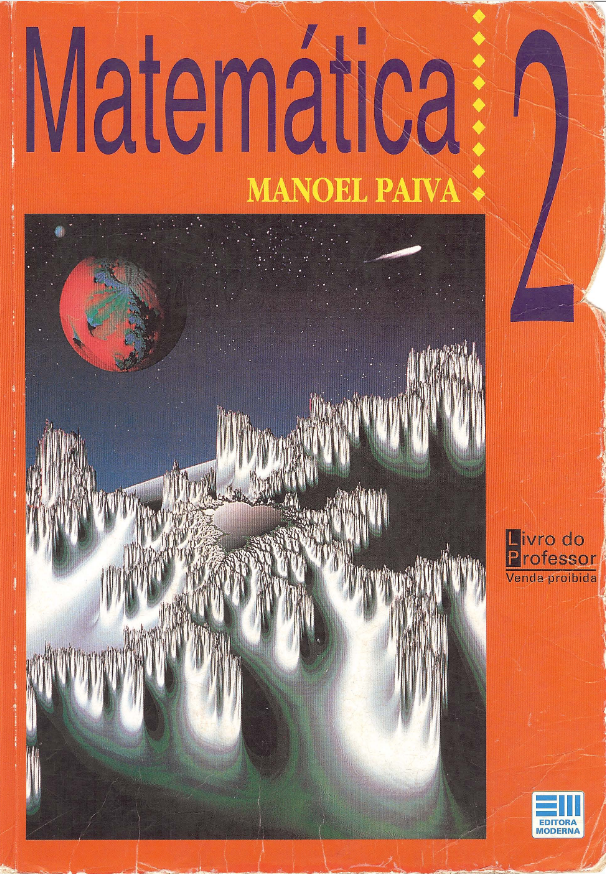
\includegraphics[width=0.5\linewidth]{imagens/Capa-Livro-Matematica-Volume-2-Manoel-Paiva-2004} 

}

\caption{Livro - Matemática Vol 3 - Manoel Paiva, 2004 (Ed. Moderna, 1.ed.)}\label{fig:unnamed-chunk-9}
\end{figure}

\begin{longtable}[]{@{}ll@{}}
\toprule()
Capítulo & Descrição \\
\midrule()
\endhead
32 & O conceito de probabilidade \\
33 & Propriedade da probabilidade \\
34 & Adição de probabilidade \\
35 & Probabilidade condicional \\
36 & Multiplicação de probabilidade \\
\bottomrule()
\end{longtable}

\hypertarget{capuxedtulo-21---anuxe1lise-combinatuxf3ria-muxe9todos-de-contagem-2}{%
\section{Capítulo 21 - Análise combinatória (Métodos de contagem)}\label{capuxedtulo-21---anuxe1lise-combinatuxf3ria-muxe9todos-de-contagem-2}}

\hypertarget{subseuxe7uxe3o-numerada-1-5}{%
\subsection{Subseção Numerada 1}\label{subseuxe7uxe3o-numerada-1-5}}

Lorem ipsum. Lorem ipsum. Lorem ipsum. Lorem ipsum. Lorem ipsum. Lorem ipsum. Lorem ipsum. Lorem ipsum. Lorem ipsum. Lorem ipsum. Lorem ipsum. Lorem ipsum. Lorem ipsum. Lorem ipsum. Lorem ipsum. Lorem ipsum. Lorem ipsum. Lorem ipsum. Lorem ipsum.

\hypertarget{exercuxedcios-do-capuxedtulo-21-1}{%
\subsection{Exercícios do Capítulo 21}\label{exercuxedcios-do-capuxedtulo-21-1}}

Lorem ipsum. Lorem ipsum. Lorem ipsum. Lorem ipsum. Lorem ipsum. Lorem ipsum. Lorem ipsum. Lorem ipsum. Lorem ipsum. Lorem ipsum. Lorem ipsum. Lorem ipsum. Lorem ipsum. Lorem ipsum. Lorem ipsum. Lorem ipsum. Lorem ipsum. Lorem ipsum. Lorem ipsum.

\hypertarget{seuxe7uxe3o-nuxe3o-numerada-3-5}{%
\subsection*{Seção não Numerada 3}\label{seuxe7uxe3o-nuxe3o-numerada-3-5}}
\addcontentsline{toc}{subsection}{Seção não Numerada 3}

Lorem ipsum. Lorem ipsum. Lorem ipsum. Lorem ipsum. Lorem ipsum. Lorem ipsum. Lorem ipsum. Lorem ipsum. Lorem ipsum. Lorem ipsum. Lorem ipsum. Lorem ipsum. Lorem ipsum. Lorem ipsum. Lorem ipsum. Lorem ipsum. Lorem ipsum. Lorem ipsum. Lorem ipsum.
eção 02

\hypertarget{capuxedtulo-22---princuxedpio-aditivo-da-contagem-2}{%
\section{Capítulo 22 - Princípio aditivo da contagem}\label{capuxedtulo-22---princuxedpio-aditivo-da-contagem-2}}

\hypertarget{subseuxe7uxe3o-numerada-1-6}{%
\subsection{Subseção Numerada 1}\label{subseuxe7uxe3o-numerada-1-6}}

Lorem ipsum. Lorem ipsum. Lorem ipsum. Lorem ipsum. Lorem ipsum. Lorem ipsum. Lorem ipsum. Lorem ipsum. Lorem ipsum. Lorem ipsum. Lorem ipsum. Lorem ipsum. Lorem ipsum. Lorem ipsum. Lorem ipsum. Lorem ipsum. Lorem ipsum. Lorem ipsum. Lorem ipsum.

\hypertarget{exercuxedcios-do-capuxedtulo-22-2}{%
\subsection{Exercícios do Capítulo 22}\label{exercuxedcios-do-capuxedtulo-22-2}}

Lorem ipsum. Lorem ipsum. Lorem ipsum. Lorem ipsum. Lorem ipsum. Lorem ipsum. Lorem ipsum. Lorem ipsum. Lorem ipsum. Lorem ipsum. Lorem ipsum. Lorem ipsum. Lorem ipsum. Lorem ipsum. Lorem ipsum. Lorem ipsum. Lorem ipsum. Lorem ipsum. Lorem ipsum.

\hypertarget{seuxe7uxe3o-nuxe3o-numerada-3-6}{%
\subsection*{Seção não Numerada 3}\label{seuxe7uxe3o-nuxe3o-numerada-3-6}}
\addcontentsline{toc}{subsection}{Seção não Numerada 3}

Lorem ipsum. Lorem ipsum. Lorem ipsum. Lorem ipsum. Lorem ipsum. Lorem ipsum. Lorem ipsum. Lorem ipsum. Lorem ipsum. Lorem ipsum. Lorem ipsum. Lorem ipsum. Lorem ipsum. Lorem ipsum. Lorem ipsum. Lorem ipsum. Lorem ipsum. Lorem ipsum. Lorem ipsum.

\hypertarget{capuxedtulo-23---arranjo-simples-2}{%
\section{Capítulo 23 - Arranjo simples}\label{capuxedtulo-23---arranjo-simples-2}}

\hypertarget{subseuxe7uxe3o-numerada-1-7}{%
\subsection{Subseção Numerada 1}\label{subseuxe7uxe3o-numerada-1-7}}

Lorem ipsum. Lorem ipsum. Lorem ipsum. Lorem ipsum. Lorem ipsum. Lorem ipsum. Lorem ipsum. Lorem ipsum. Lorem ipsum. Lorem ipsum. Lorem ipsum. Lorem ipsum. Lorem ipsum. Lorem ipsum. Lorem ipsum. Lorem ipsum. Lorem ipsum. Lorem ipsum. Lorem ipsum.

\hypertarget{exercuxedcios-do-capuxedtulo-23-2}{%
\subsection{Exercícios do Capítulo 23}\label{exercuxedcios-do-capuxedtulo-23-2}}

Lorem ipsum. Lorem ipsum. Lorem ipsum. Lorem ipsum. Lorem ipsum. Lorem ipsum. Lorem ipsum. Lorem ipsum. Lorem ipsum. Lorem ipsum. Lorem ipsum. Lorem ipsum. Lorem ipsum. Lorem ipsum. Lorem ipsum. Lorem ipsum. Lorem ipsum. Lorem ipsum. Lorem ipsum.

\hypertarget{seuxe7uxe3o-nuxe3o-numerada-3-7}{%
\subsection*{Seção não Numerada 3}\label{seuxe7uxe3o-nuxe3o-numerada-3-7}}
\addcontentsline{toc}{subsection}{Seção não Numerada 3}

Lorem ipsum. Lorem ipsum. Lorem ipsum. Lorem ipsum. Lorem ipsum. Lorem ipsum. Lorem ipsum. Lorem ipsum. Lorem ipsum. Lorem ipsum. Lorem ipsum. Lorem ipsum. Lorem ipsum. Lorem ipsum. Lorem ipsum. Lorem ipsum. Lorem ipsum. Lorem ipsum. Lorem ipsum.

\begin{itemize}
\tightlist
\item
\end{itemize}

  \bibliography{referencias.bib,packages.bib}

\end{document}
